\documentclass[12pt]{article}
\usepackage[utf8]{inputenc}
\usepackage[T1]{fontenc}
\usepackage{amsmath}
\usepackage{amsfonts}
\usepackage{amssymb}
\usepackage[version=4]{mhchem}
\usepackage{stmaryrd}
\usepackage{graphicx}
\usepackage[export]{adjustbox}
\graphicspath{ {./images/} }
\setlength{\parindent}{0pt}
\usepackage{setspace}
\setstretch{1.5}

\author{Qixiang Fang}
\date{\today}


\begin{document}

\section*{M032064}

Ann and Jenny divide $560$ zeds between them. If Jenny gets $\frac{3}{8}$ of the money, how many zeds will Ann get?

\newpage
\section*{M032094}

$\frac{4}{100}+\frac{3}{1000}=$

[A] 0.043

[B] 0.1043

[C] 0.403

[D] 0.43

\newpage
\section*{M032166}

Which of these is the BEST estimate of $\frac{7.21 \times 3.86}{10.09} ?$

[A] $\frac{7 \times 3}{10}$

[B] $\frac{7 \times 4}{10}$

[C] $\frac{7 \times 3}{11}$

[D] $\frac{7 \times 4}{11}$



\newpage
\section*{M032595}

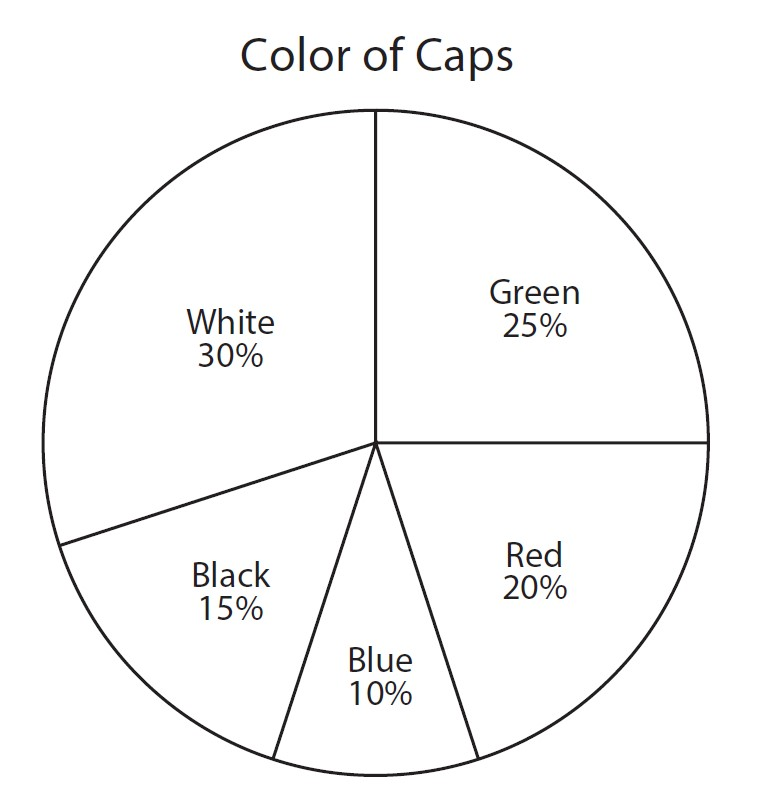
\includegraphics[width=0.5\textwidth]{2024_02_20_828ebc9d68bcc1fbb223g-04}

The pie chart shows the percentage of caps for sale at a sporting goods store. If there are 200 caps, what is the total number of caps that are either white or green?

[A] 55

[B] 100

[C] 110

[D] 145

\newpage
\section*{M032626}

Which of these shows how 36 can be expressed as a product of prime factors?

[A] $6 \times 6$

[B] $4 \times 9$

[C] $4 \times 3 \times 3$

[D] $2 \times 2 \times 3 \times 3$

\newpage
\section*{M032662}

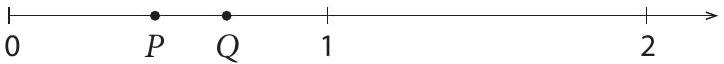
\includegraphics[max width=0.5\textwidth]{2024_02_20_828ebc9d68bcc1fbb223g-06(1)}

$P$ and $Q$ represent two fractions on the number line above.

$P \times Q=N$.

Which of these shows the location of $N$ on the number line?

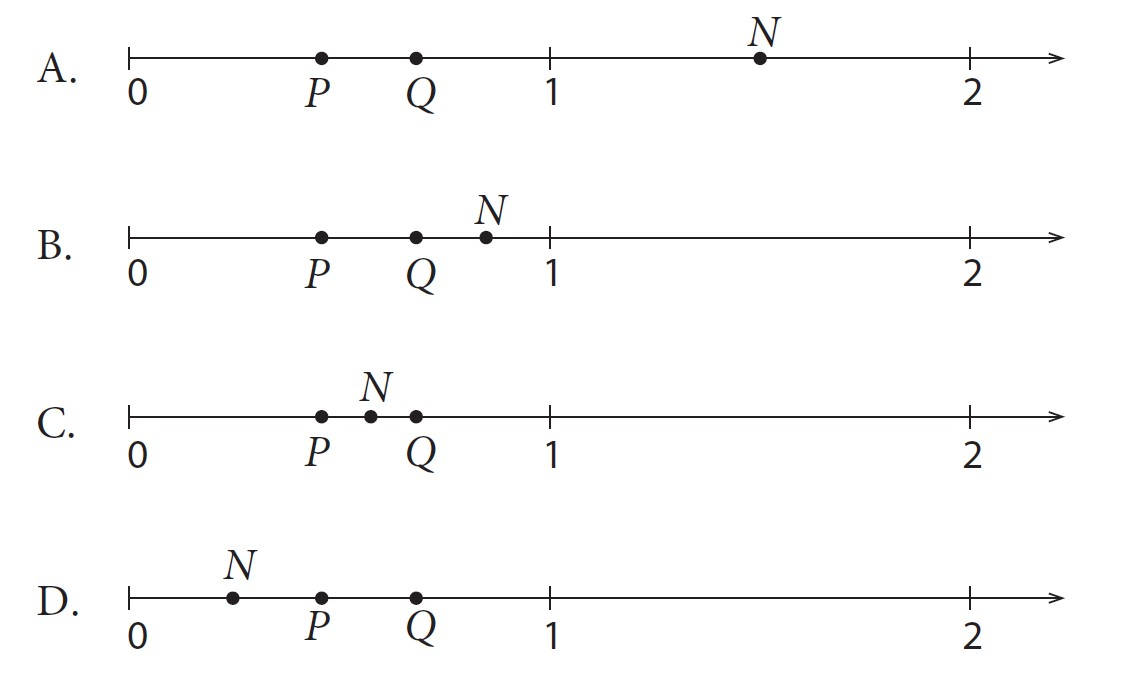
\includegraphics[max width=0.5\textwidth]{2024_02_20_828ebc9d68bcc1fbb223g-06(2)}

\newpage
\section*{M032725}

Write $3 \frac{5}{6}$ in decimal form, rounded to 2 decimal places.

\newpage
\section*{M042002}

Place the four digits $3,5,7$, and 9 into the boxes below in the positions that would give the greatest result when the two numbers are multiplied.

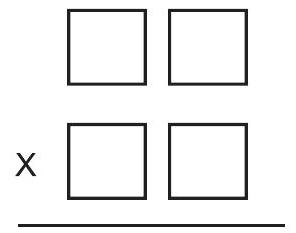
\includegraphics[max width=0.5\textwidth]{2024_02_20_828ebc9d68bcc1fbb223g-08}

\newpage
\section*{M042016}

Look at this table:


\begin{tabular}{|c|c|c|c|c|c|}
\hline
$4^{1}$ & $4^{2}$ & $4^{3}$ & $4^{4}$ & $4^{5}$ & $4^{6}$ \\
\hline
4 & 16 & 64 & 256 & 1,024 & 4,096 \\
\hline
\end{tabular}


Use the table to express the value of $256 \times 4,096$ as a power of 4 .

[A] $4^{10}$

[B] $4^{16}$

[C] $4^{20}$

[D] $4^{24}$

\newpage
\section*{M042024}

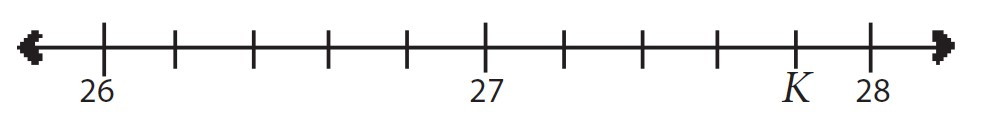
\includegraphics[max width=0.9\textwidth]{2024_02_20_828ebc9d68bcc1fbb223g-10}

Which number does $K$ represent on this number line?

[A] 27.4

[B] 27.8

[C] 27.9

[D] 28.2

\newpage
\section*{M042031}

The fractions $\frac{4}{14}$ and $\frac{\square}{21}$ are equivalent.

What is the value of $\square$ ?

[A] 6

[B] 7

[C] 11

[D] 14

\newpage
\section*{M042032}

Which fraction is equivalent to 0.125 ?

[A] $\frac{125}{100}$

[B] $\frac{125}{1,000}$

[C] $\frac{125}{10,000}$

[D] $\frac{125}{100,000}$

\newpage
\section*{M042041}

A workman cut off $\frac{1}{5}$ of a pipe. The piece he cut off was 3 meters long.

How many meters long was the original pipe?

[A] $8 \mathrm{~m}$

[B] $12 \mathrm{~m}$

[C] $15 \mathrm{~m}$

[D] $18 \mathrm{~m}$

\newpage
\section*{M042059}

Peter, James, and Andrew each had 20 tries at throwing balls into a basket.

Complete the missing boxes below.


\begin{tabular}{lrr}
Name & \begin{tabular}{c}
Number of \\
Successful Shots \\
\end{tabular} & \begin{tabular}{c}
Percentag \\
Successful Shots \\
\end{tabular} \\
Peter & 10 out of 20 & $50 \%$ \\
James & 15 out of 20 & $\square$ \\
 &  &  \\
Andrew & $\square$ out of 20 &  $80 \%$ \\
\end{tabular}


\newpage
\section*{M042186}

Here is a pattern:

$3-3=0$

$3-2=1$

$3-1=2$

$3-0=3$

What will the next line in the pattern be?



\newpage
\section*{M052061}

Kim is packing eggs into boxes.

Each box holds 6 eggs.

She has 94 eggs.

What is the smallest number of boxes she needs to pack all the eggs?

\newpage
\section*{M052214}

Which of these number sentences is true?

[A] $\frac{3}{10}$ of $50=50 \%$ of 3

[B] $3 \%$ of $50=6 \%$ of 100

[C] $50 \div 30=30 \div 50$

[D] $\frac{3}{10} \times 50=\frac{5}{10} \times 30$

\newpage
\section*{M052216}

Which number is equal to $\frac{3}{5} ?$

[A] 0.8

[B] 0.6

[C] 0.53

[D] 0.35

\newpage
\section*{M052228}

Which shows a correct method for finding $\frac{1}{3}-\frac{1}{4} ?$

[A] $\frac{1-1}{4-3}$

[B] $\frac{1}{4-3}$

[C] $\frac{3-4}{3 \times 4}$

[D] $\frac{4-3}{3 \times 4}$

\newpage
\section*{M052231}

$42.65+5.748=$

\newpage
\section*{M032047}

What is the sum of the three consecutive whole numbers with $2 n$ as the middle number?

[A] $6 n+3$

[B] $6 n$

[C] $6 n-1$

[D] $6 n-3$

\newpage
\section*{M032295}

There were $m$ boys and $n$ girls in a parade. Each person carried 2 balloons. Which of these expressions represents the total number of balloons that were carried in the parade?

[A] $2(m+n)$

[B] $2+(m+n)$

[C] $2 m+n$

[D] $m+2 n$

\newpage
\section*{M032352}


\begin{tabular}{|c|c|}
\hline
\begin{tabular}{c}
Bush \\
height $(\mathbf{c m})$ \\
\end{tabular} & \begin{tabular}{c}
Shadow \\
length $(\mathbf{c m})$ \\
\end{tabular} \\
\hline
20 & 16 \\
\hline
40 & 32 \\
\hline
60 & 48 \\
\hline
80 & 64 \\
\hline
\end{tabular}


The table above shows the shadow lengths of four bushes of different heights at $10 \mathrm{a} . \mathrm{m}$. What is the shadow length at $10 \mathrm{a} . \mathrm{m}$. of a bush that has a height of 50 centimeters?

[A] $36 \mathrm{~cm}$

[B] $38 \mathrm{~cm}$

[C] $40 \mathrm{~cm}$

[D] $42 \mathrm{~cm}$

\newpage
\section*{M032419}

Which of these could represent the expression $2 x+3 x$ ?

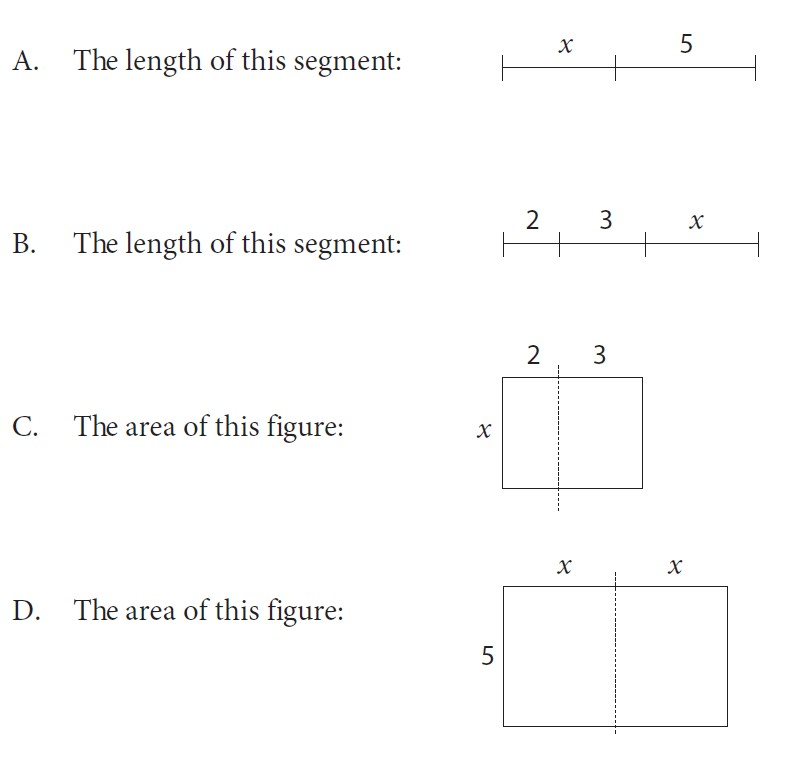
\includegraphics[max width=0.8\textwidth]{2024_02_20_828ebc9d68bcc1fbb223g-24}

\newpage
\section*{M032424}

Jo has three metal blocks. The weight of each block is the same. When she weighed one block against 8 grams, this is what happened.

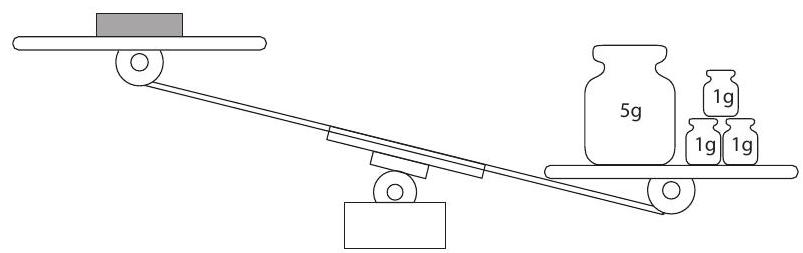
\includegraphics[max width=0.8\textwidth]{2024_02_20_828ebc9d68bcc1fbb223g-25}

When she weighed all three blocks against 20 grams, this is what happened.

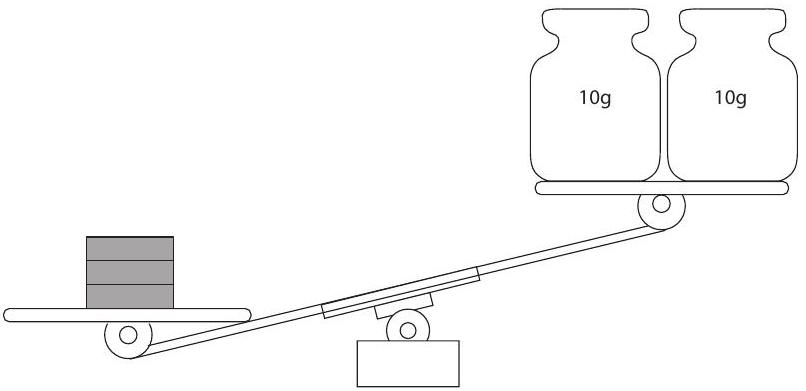
\includegraphics[max width=0.8\textwidth]{2024_02_20_828ebc9d68bcc1fbb223g-25(1)}

Which of the following could be the weight of one metal block?

[A] $5 \mathrm{~g}$

[B] $6 \mathrm{~g}$

[C] $7 \mathrm{~g}$

[D] $8 \mathrm{~g}$

\newpage
\section*{M032477}

The taxi company has a basic charge of 25 zeds and a charge of 0.2 zeds for each kilometer the taxi is driven. Which of these represents the cost in zeds to hire a taxi for a trip of $n$ kilometers?

[A] $25+0.2 n$

[B] $25 \times 0.2 n$

[C] $0.2 \times(25+n)$

[D] $0.2 \times 25+n$

\newpage
\section*{M032538}

Use the formula $y=100-\frac{100}{1+t}$ to find the value of $y$ when $t=9$.

\newpage
\section*{M032673}

If $t$ is a number between 6 and 9 , then $t+5$ is between what two numbers?

[A] 1 and 4

[B] 10 and 13

[C] 11 and 14

[D] 30 and 45

\newpage
\section*{M032683}

Simplify the expression $\frac{3 x}{8}+\frac{x}{4}+\frac{x}{2}$. Show your work.

\newpage
\section*{M032738}

What does $x y+1$ mean?

[A] Add 1 to $y$, then multiply by $x$.

[B] Multiply $x$ and $y$ by 1 .

[C] Add $x$ to $y$, then add 1 .

[D] Multiply $x$ by $y$, then add 1 .

\newpage
\section*{M032757}

Pat has red tiles and black tiles. Pat uses the tiles to make square shapes.

The $3 \times 3$ shape has 1 black tile and 8 red tiles.

The $4 \times 4$ shape has 4 black tiles and 12 red tiles.

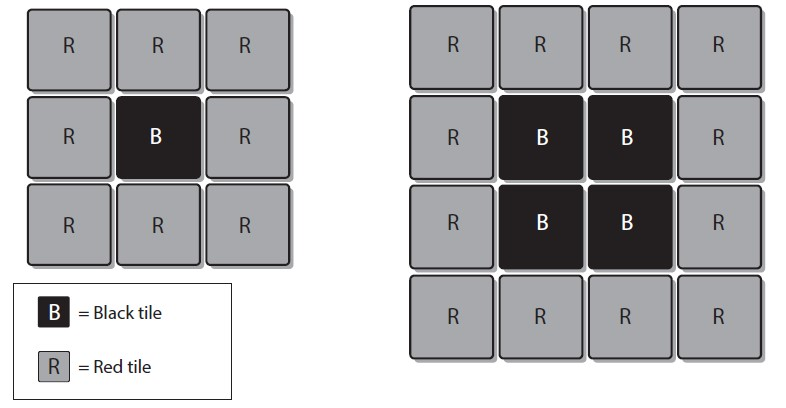
\includegraphics[max width=\textwidth]{2024_02_20_828ebc9d68bcc1fbb223g-31}

The table below shows the number of tiles for the first three shapes Pat made. Pat continued making shapes using this pattern. Complete the table for the $6 \times 6$ and $7 \times 7$ shapes.


\begin{tabular}{|c|c|c|c|}
\hline
Shape & \begin{tabular}{c}
Number of \\
Black Tiles \\
\end{tabular} & \begin{tabular}{c}
Number of \\
Red Tiles \\
\end{tabular} & \begin{tabular}{c}
Total Number \\
of Tiles \\
\end{tabular} \\
\hline
$3 \times 3$ & 1 & 8 & 9 \\
\hline
$4 \times 4$ & 4 & 12 & 16 \\
\hline
$5 \times 5$ & 9 & 16 & 25 \\
\hline
$6 \times 6$ & 16 &  &  \\
\hline
$7 \times 7$ & 25 &  &  \\
\hline
\end{tabular}


\newpage
\section*{M032760A}

Pat has red tiles and black tiles. Pat uses the tiles to make square shapes.

The $3 \times 3$ shape has 1 black tile and 8 red tiles.

The $4 \times 4$ shape has 4 black tiles and 12 red tiles.

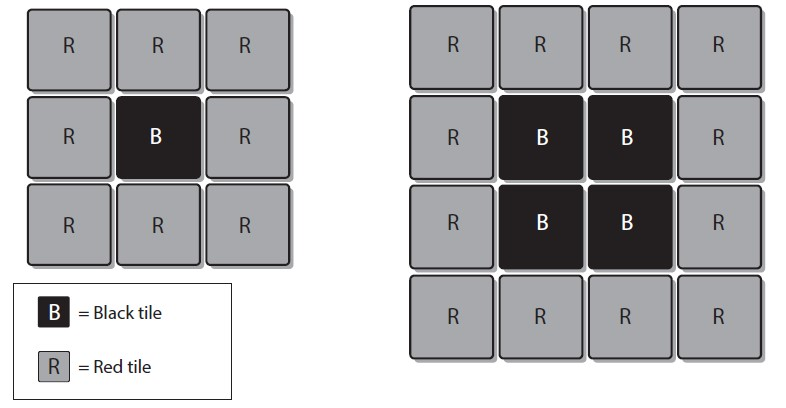
\includegraphics[max width=\textwidth]{2024_02_20_828ebc9d68bcc1fbb223g-31}

The table below shows the number of tiles for the first three shapes Pat made. Pat continued making shapes using this pattern. 


\begin{tabular}{|c|c|c|c|}
\hline
Shape & \begin{tabular}{c}
Number of \\
Black Tiles \\
\end{tabular} & \begin{tabular}{c}
Number of \\
Red Tiles \\
\end{tabular} & \begin{tabular}{c}
Total Number \\
of Tiles \\
\end{tabular} \\
\hline
$3 \times 3$ & 1 & 8 & 9 \\
\hline
$4 \times 4$ & 4 & 12 & 16 \\
\hline
$5 \times 5$ & 9 & 16 & 25 \\
\hline
\end{tabular}


Pat made a shape with a total of 64 tiles. How many were black and how many were red?

\newpage
\section*{M032760B}

Pat has red tiles and black tiles. Pat uses the tiles to make square shapes.

The $3 \times 3$ shape has 1 black tile and 8 red tiles.

The $4 \times 4$ shape has 4 black tiles and 12 red tiles.

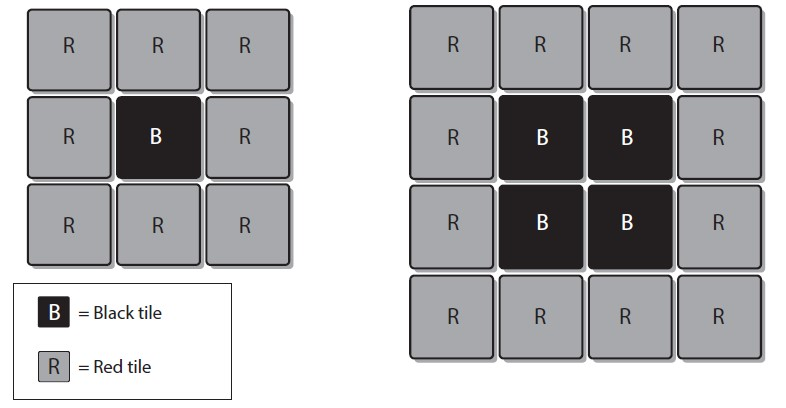
\includegraphics[max width=\textwidth]{2024_02_20_828ebc9d68bcc1fbb223g-31}

The table below shows the number of tiles for the first three shapes Pat made. Pat continued making shapes using this pattern. 


\begin{tabular}{|c|c|c|c|}
\hline
Shape & \begin{tabular}{c}
Number of \\
Black Tiles \\
\end{tabular} & \begin{tabular}{c}
Number of \\
Red Tiles \\
\end{tabular} & \begin{tabular}{c}
Total Number \\
of Tiles \\
\end{tabular} \\
\hline
$3 \times 3$ & 1 & 8 & 9 \\
\hline
$4 \times 4$ & 4 & 12 & 16 \\
\hline
$5 \times 5$ & 9 & 16 & 25 \\
\hline
\end{tabular}


Pat made a shape that used 49 black tiles.

How many red tiles did Pat use in that shape?

\newpage
\section*{M032760C}


Pat has red tiles and black tiles. Pat uses the tiles to make square shapes.

The $3 \times 3$ shape has 1 black tile and 8 red tiles.

The $4 \times 4$ shape has 4 black tiles and 12 red tiles.

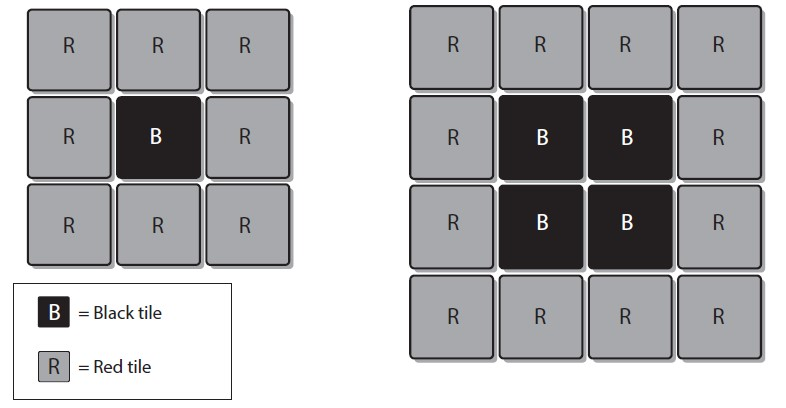
\includegraphics[max width=\textwidth]{2024_02_20_828ebc9d68bcc1fbb223g-31}

The table below shows the number of tiles for the first three shapes Pat made. Pat continued making shapes using this pattern. 


\begin{tabular}{|c|c|c|c|}
\hline
Shape & \begin{tabular}{c}
Number of \\
Black Tiles \\
\end{tabular} & \begin{tabular}{c}
Number of \\
Red Tiles \\
\end{tabular} & \begin{tabular}{c}
Total Number \\
of Tiles \\
\end{tabular} \\
\hline
$3 \times 3$ & 1 & 8 & 9 \\
\hline
$4 \times 4$ & 4 & 12 & 16 \\
\hline
$5 \times 5$ & 9 & 16 & 25 \\
\hline
\end{tabular}


Next, Pat made a shape using 44 of the red tiles. How many black tiles would Pat need to complete the black part of the shape?

\newpage
\section*{M032761}


Pat has red tiles and black tiles. Pat uses the tiles to make square shapes.

The $3 \times 3$ shape has 1 black tile and 8 red tiles.

The $4 \times 4$ shape has 4 black tiles and 12 red tiles.

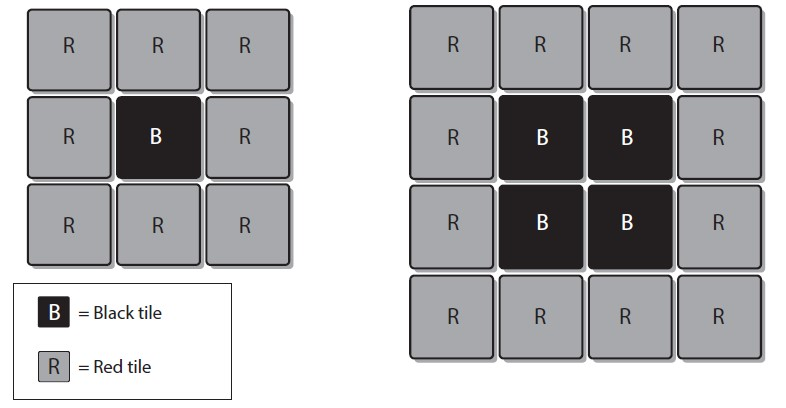
\includegraphics[max width=\textwidth]{2024_02_20_828ebc9d68bcc1fbb223g-31}

The table below shows the number of tiles for the first three shapes Pat made. Pat continued making shapes using this pattern. 


\begin{tabular}{|c|c|c|c|}
\hline
Shape & \begin{tabular}{c}
Number of \\
Black Tiles \\
\end{tabular} & \begin{tabular}{c}
Number of \\
Red Tiles \\
\end{tabular} & \begin{tabular}{c}
Total Number \\
of Tiles \\
\end{tabular} \\
\hline
$3 \times 3$ & 1 & 8 & 9 \\
\hline
$4 \times 4$ & 4 & 12 & 16 \\
\hline
$5 \times 5$ & 9 & 16 & 25 \\
\hline
\end{tabular}


Pat wanted to add a line to the table showing how to find the number of tiles needed to make a square of any size. Complete the line for shape $n \times n$ in the table below.


\begin{tabular}{|c|c|c|c|}
\hline
Shape & \begin{tabular}{c}
Number of \\
Black Tiles \\
\end{tabular} & \begin{tabular}{c}
Number of \\
Red Tiles \\
\end{tabular} & \begin{tabular}{c}
Total Number \\
of Tiles \\
\end{tabular} \\
\hline
$n \times n$ & $(n-2)^{2}$ &  &  \\
\hline
\end{tabular}


\newpage
\section*{M042067}

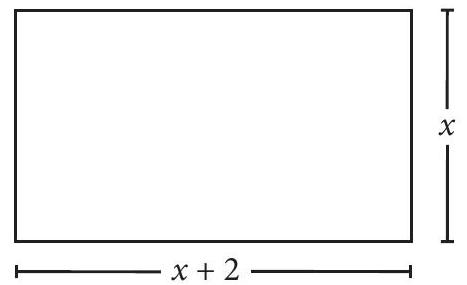
\includegraphics[max width=0.5\textwidth]{2024_02_20_828ebc9d68bcc1fbb223g-36}

What is the area of this rectangle?

[A] $x^{2}+2$

[B] $x^{2}+2 x$

[C] $2 x+2$

[D] $4 x+4$

\newpage
\section*{M042077}

Which expression is equivalent to $4(3+x)$ ?

[A] $12+x$

[B] $7+x$

[C] $12+4 x$

[D] $12 x$

\newpage
\section*{M042086}
$a+b=25$.

What is the value of $2 a+2 b+4$ ?

\newpage
\section*{M042103}

Solve this inequality.

$9 x-6<4 x+4$

\newpage
\section*{M042198A}

$$
\frac{1}{2}, \frac{2}{3}, \frac{3}{4}, \frac{4}{5}, \frac{5}{6}
$$

What is the next term in this pattern?

\newpage
\section*{M042198B}

$$
\frac{1}{2}, \frac{2}{3}, \frac{3}{4}, \frac{4}{5}, \frac{5}{6}
$$

What would term number 100 be?

\newpage
\section*{M042198C}

$$
\frac{1}{2}, \frac{2}{3}, \frac{3}{4}, \frac{4}{5}, \frac{5}{6}
$$

What would term number $n$ be?

\newpage
\section*{M042226}

$k=7$ and $l=10$.

What is the value of $P$ when $P=\frac{3 k l}{5}$ ?

\newpage
\section*{M042228}


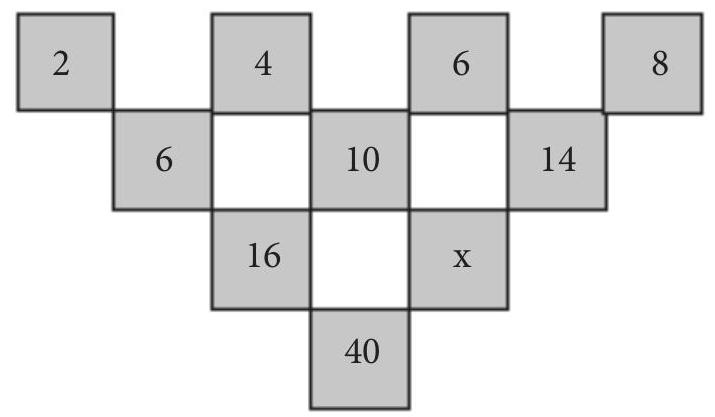
\includegraphics[max width=0.6\textwidth]{2024_02_20_828ebc9d68bcc1fbb223g-44}


What is the value of $x$ in this pattern?

\newpage
\section*{M042235}

$x+y=12$ and $2 x+5 y=36$.

What are the values of $x$ and $y$ ?

[A] $x=2, y=10$

[B] $x=4, y=8$

[C] $x=6, y=6$

[D] $x=8, y=4$

\newpage
\section*{M042236}

Which of these is equal to $3 p^{2}+2 p+2 p^{2}+p$ ?

[A] $8 p$

[B] $8 p^{2}$

[C] $5 p^{2}+3 p$

[D] $7 p^{2}+p$

\newpage
\section*{M042245}

$(0,-1),(1,3)$

Which equation is satisfied by BOTH of these pairs of numbers $(x, y)$ ?

[A] $x+y=-1$

[B] $2 x+y=5$

[C] $3 x-y=0$

[D] $4 x-y=1$

\newpage
\section*{M052002}

A piece of wood was $40 \mathrm{~cm}$ long.

It was cut into 3 pieces.

The lengths in $\mathrm{cm}$ are

$2 x-5$

$x+7$

$x+6$

What is the length of the longest piece?

\newpage
\section*{M052173}


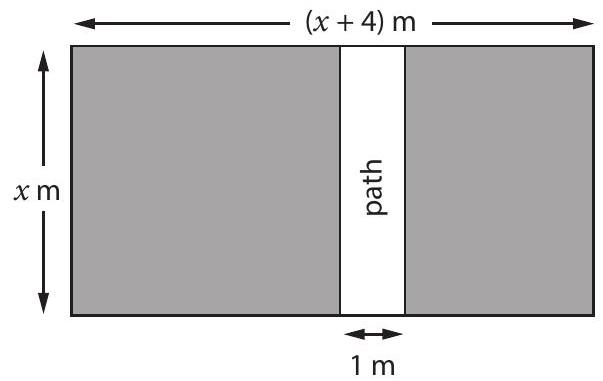
\includegraphics[max width=0.7\textwidth]{2024_02_20_828ebc9d68bcc1fbb223g-49}


This is a diagram of a rectangular garden.

The white area is a rectangular path that is 1 meter wide.

Which expression shows the area of the shaded portion of the garden in $\mathrm{m}^{2}$~ ?

[A] $x^{2}+3 x$

[B] $x^{2}+4 x$

[C] $x^{2}+4 x-1$

[D] $x^{2}+3 x-1$

\newpage
\section*{M052302}

$y=\frac{a+b}{c}$

$a=8, b=6$, and $c=2$

What is the value of $y$ ?

[A] 7

[B] 10

[C] 11

[D] 14

\newpage
\section*{M032100}


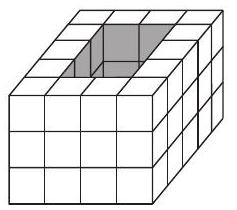
\includegraphics[max width=0.3\textwidth]{2024_02_20_828ebc9d68bcc1fbb223g-51}


The figure above shows a shape made up of cubes that are all the same size. There is a hole all the way through the shape. How many cubes would be needed to fill the hole?

[A] 6

[B] 12

[C] 15

[D] 18

\newpage
\section*{M032116}

The area of a square is $144 \mathrm{~cm}^{2}$. What is the perimeter of the square?

[A] $12 \mathrm{~cm}$

[B] $48 \mathrm{~cm}$

[C] $288 \mathrm{~cm}$

[D] $576 \mathrm{~cm}$

\newpage
\section*{M032324}

Points $A, B$, and $C$ lie on a line and $B$ is between $A$ and $C$. If $A B=10 \mathrm{~cm}$ and $B C=5.2 \mathrm{~cm}$, what is the distance between the midpoints of $A B$ and $B C$ ?

[A] $2.4 \mathrm{~cm}$

[B] $2.6 \mathrm{~cm}$

[C] $5.0 \mathrm{~cm}$

[D] $7.6 \mathrm{~cm}$

\newpage
\section*{M032331}

How many degrees does a minute hand of a clock turn through from 6:20 a.m. to 8:00 a.m. on the same day?

[A] $680^{\circ}$

[B] $600^{\circ}$

[C] $540^{\circ}$

[D] $420^{\circ}$

\newpage
\section*{M032397}


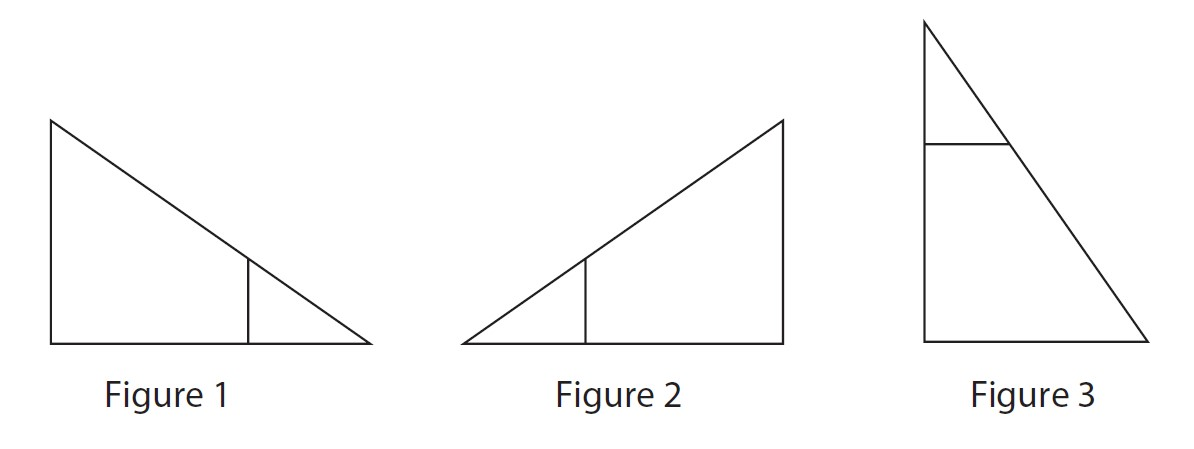
\includegraphics[max width=0.9\textwidth]{2024_02_20_828ebc9d68bcc1fbb223g-55}

Which of these transformations, taken in order, can be used so that Figure 1 above becomes Figure 2 and then Figure 3?

[A] reflection and then translation

[B] reflection and then $\frac{1}{4}$ turn rotation clockwise

[C] $\frac{1}{2}$ turn rotation and then translation

[D] $\frac{1}{4}$ turn rotation counterclockwise and then reflection

\newpage
\section*{M032398}


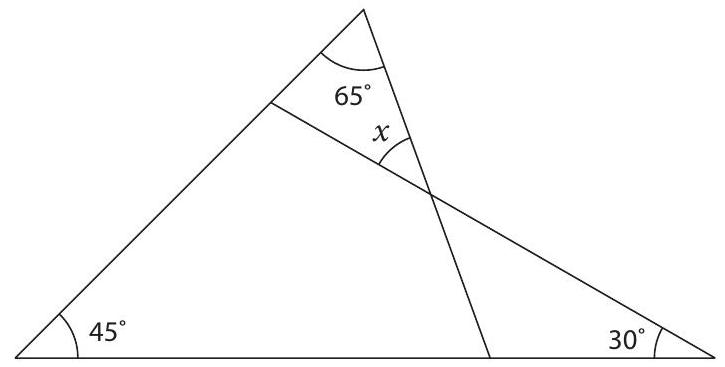
\includegraphics[max width=0.7\textwidth]{2024_02_20_828ebc9d68bcc1fbb223g-56}


In the figure above, what is the value of $x$ ?

[A] $30^{\circ}$

[B] $40^{\circ}$

[C] $45^{\circ}$

[D] $65^{\circ}$


\newpage
\section*{M032402}


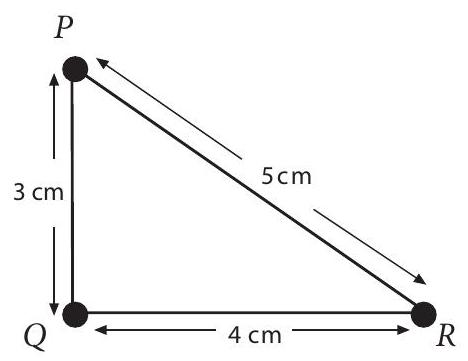
\includegraphics[max width=0.5\textwidth]{2024_02_20_828ebc9d68bcc1fbb223g-57}


Which of these is the reason that triangle $P Q R$ is a right angle triangle?

[A] $3^{2}+4^{2}=5^{2}$

[B] $5<3+4$

[C] $3+4=12-5$

[D] $3>5-4$

\newpage
\section*{M032623}


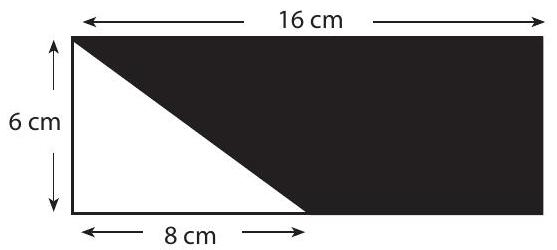
\includegraphics[max width=0.5\textwidth]{2024_02_20_828ebc9d68bcc1fbb223g-58}


In the figure above, what is the area of the shaded region in $\mathrm{cm}^{2}$ ?

[A] 24

[B] 44

[C] 48

[D] 72

\newpage
\section*{M032679}


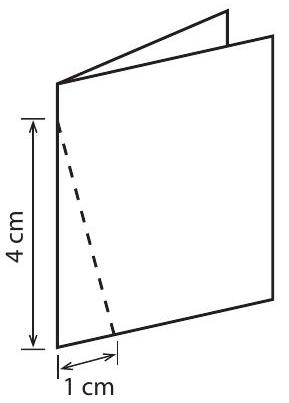
\includegraphics[max width=0.25\textwidth]{2024_02_20_828ebc9d68bcc1fbb223g-59}


A piece of paper in the shape of a rectangle is folded in half as shown in the figure above. It is then cut along the dotted line, and the small piece that is cut is opened. What is the shape of the cutout figure?

[A] an isosceles triangle

[B] two isosceles triangles

[C] a right triangle

[D] an equilateral triangle

\newpage
\section*{M032692}


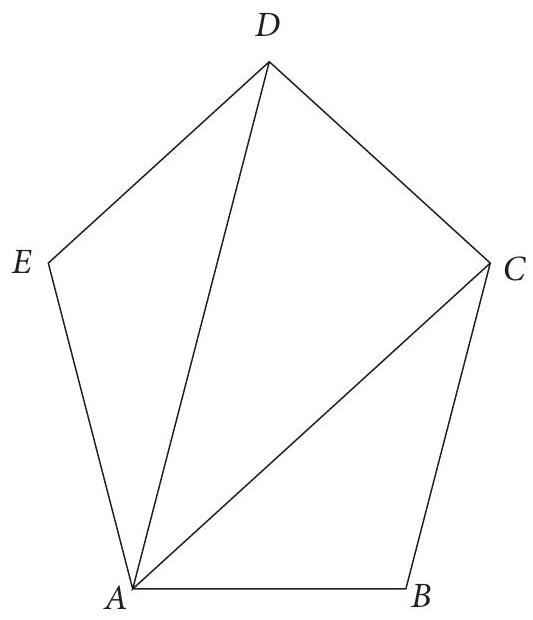
\includegraphics[max width=0.5\textwidth]{2024_02_20_828ebc9d68bcc1fbb223g-60}


What is the sum of all the interior angles of pentagon $A B C D E$ ? Show your work.

\newpage
\section*{M032734}


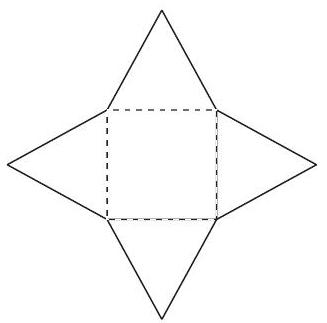
\includegraphics[max width=0.2\textwidth]{2024_02_20_828ebc9d68bcc1fbb223g-61(1)}


The shape shown above is cut out of cardboard. The triangle flaps are then folded up along the dotted lines until they touch the edges of the flaps next to them.

Complete the diagram below to show what the shape would look like when viewed from directly above.


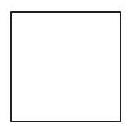
\includegraphics[max width=0.2\textwidth]{2024_02_20_828ebc9d68bcc1fbb223g-61}


\newpage
\section*{M042150}

Which shape has a line of symmetry?

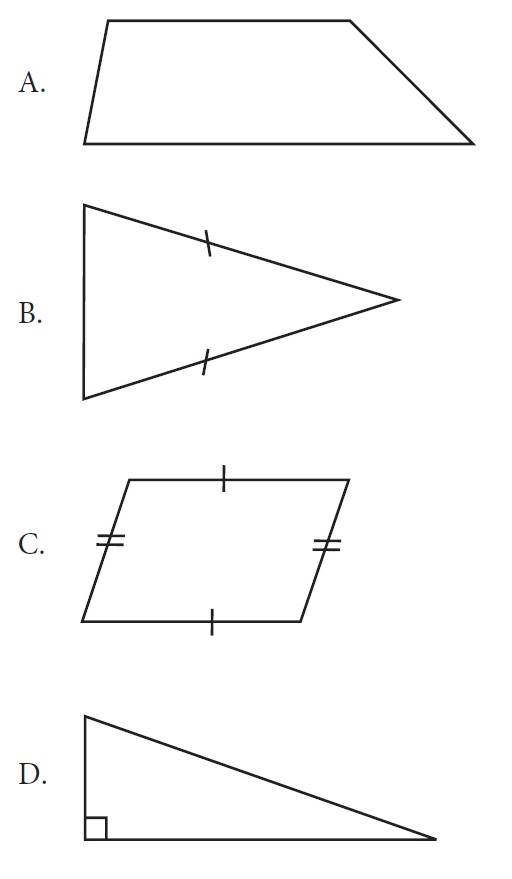
\includegraphics[max width=0.3\textwidth]{2024_02_20_828ebc9d68bcc1fbb223g-62}

\newpage
\section*{M042152}


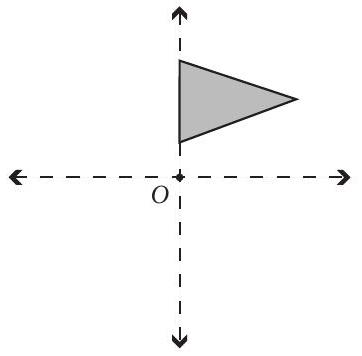
\includegraphics[max width=0.3\textwidth]{2024_02_20_828ebc9d68bcc1fbb223g-63}


Which of these shows the result of a half-turn clockwise around point $O$ ?

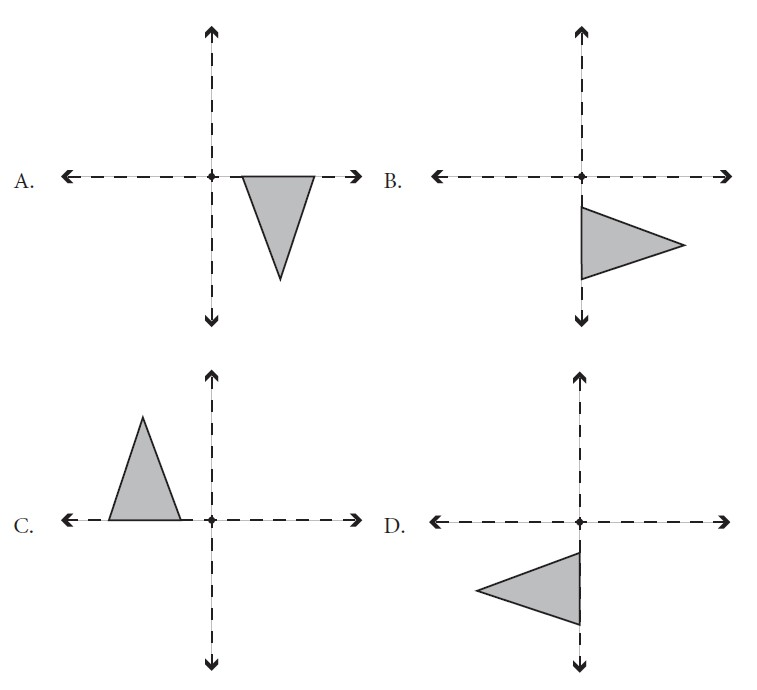
\includegraphics[max width=0.8\textwidth]{2024_02_20_828ebc9d68bcc1fbb223g-63(2)}

\newpage
\section*{M042201}


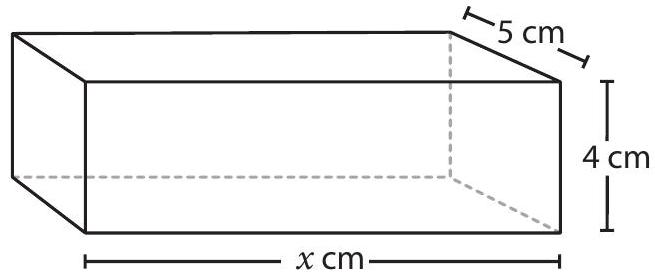
\includegraphics[max width=0.6\textwidth]{2024_02_20_828ebc9d68bcc1fbb223g-64}


The volume of the rectangular box is $200 \mathrm{~cm}^{3}$. What is the value of $x$ ?

\newpage
\section*{M042270}

The length of side of each of the small squares represents $1 \mathrm{~cm}$. Draw an isosceles triangle with a base of $4 \mathrm{~cm}$ and a height of $5 \mathrm{~cm}$.

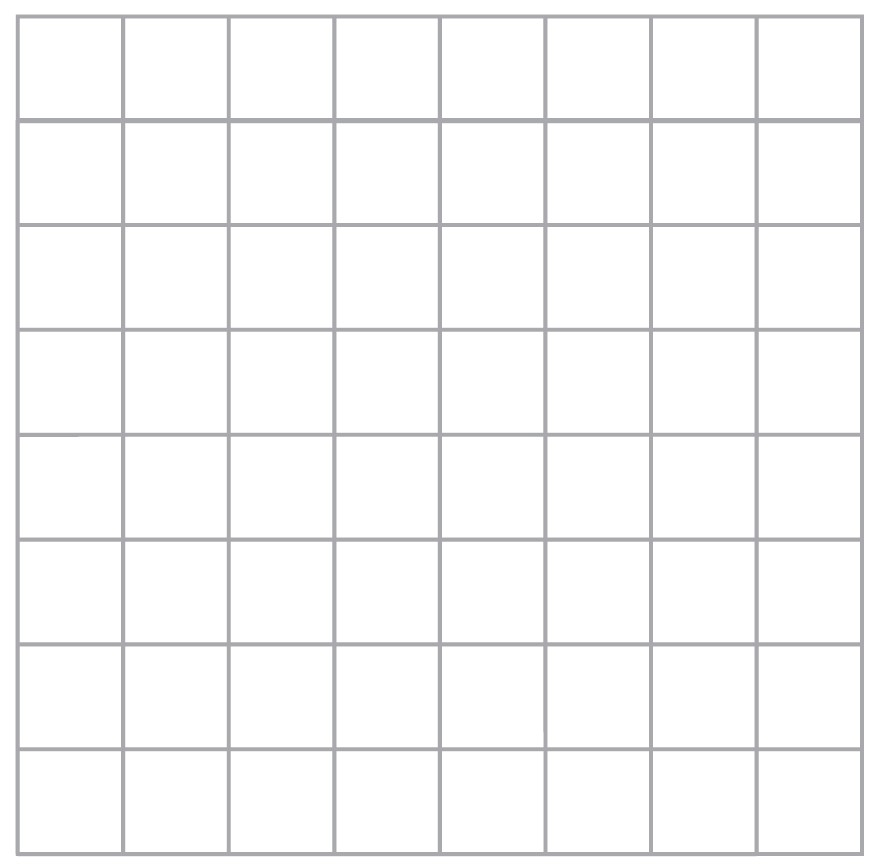
\includegraphics[max width=0.5\textwidth]{2024_02_20_828ebc9d68bcc1fbb223g-65}

\newpage
\section*{M042300Z}

The diagram shows a system for locating points


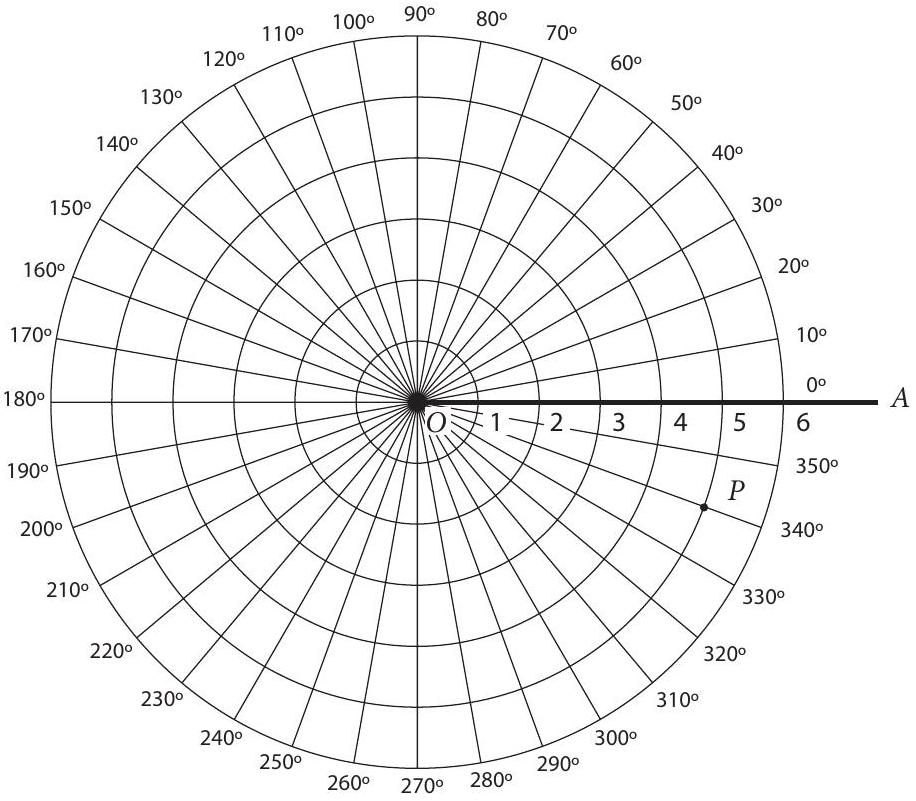
\includegraphics[max width=0.8\textwidth]{2024_02_20_828ebc9d68bcc1fbb223g-66}


In this system, the position of a point $P$ is described by its distance from origin, $O$, and the amount of counterclockwise turn from a baseline $O A$ to $O P$. Thus, the coordinates of $P$ are $\left(5,340^{\circ}\right)$.

1. Mark the points $B\left(3,30^{\circ}\right)$ and $C\left(4,120^{\circ}\right)$ on the graph above.

2. Draw the angle $B O C$. What is the measure of angle $B O C$ ?

Angle $B O C=\rule{3cm}{0.15mm}^{\circ}$

\newpage
\section*{M052084}

The perimeter of a square is $36 \mathrm{~cm}$.

What is the area of this square?

[A] $81 \mathrm{~cm}^{2}$

[B] $36 \mathrm{~cm}^{2}$

[C] $24 \mathrm{~cm}^{2}$

[D] $18 \mathrm{~cm}^{2}$

\newpage
\section*{M052206}

Ryan is packing books into a rectangular box.

All the books are the same size.


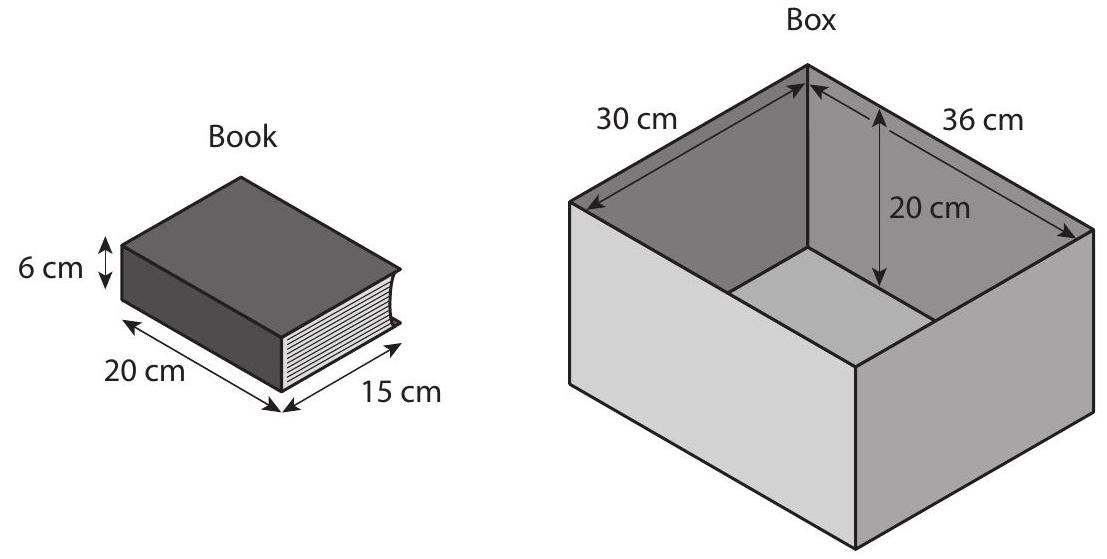
\includegraphics[max width=\textwidth]{2024_02_20_828ebc9d68bcc1fbb223g-68}


What is the largest number of books that will fit inside the box?

\newpage
\section*{M052362}


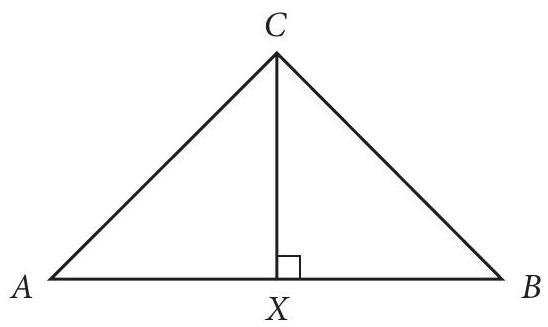
\includegraphics[max width=0.5\textwidth]{2024_02_20_828ebc9d68bcc1fbb223g-69}


In this triangle:

$A C=B C$

$A B$ is twice as long as $C X$.

What is the size of angle $B$ ?

\newpage
\section*{M052408}


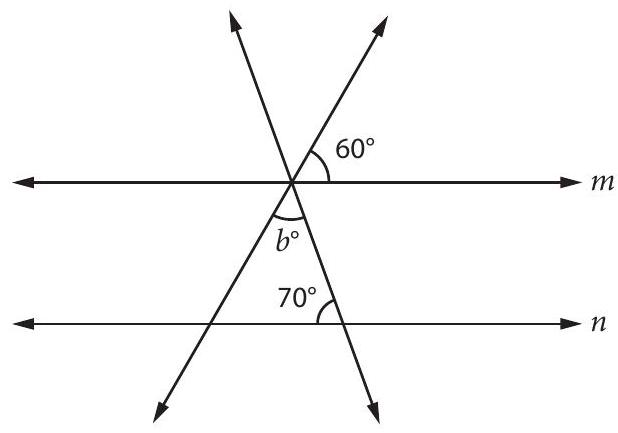
\includegraphics[max width=0.5\textwidth]{2024_02_20_828ebc9d68bcc1fbb223g-70}


Lines $m$ and $n$ are parallel.

What is the value of $b$ ?

\newpage
\section*{M032132}

A machine has 100 candies and dispenses a candy when a lever is turned. The machine has the same number of blue, pink, yellow, and green candies all mixed together. Megan turned the lever and obtained a pink candy. Peter turned the lever next.

How likely is it that Peter will get a pink candy?

[A] It is certain that his candy will be pink.

[B] It is more likely than it was for Megan.

[C] It is exactly as likely as it was for Megan.

[D] It is less likely than it was for Megan.

\newpage
\section*{M032507}


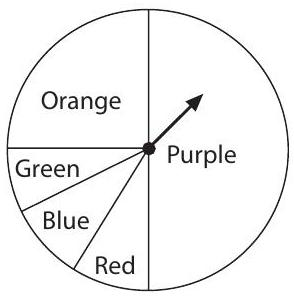
\includegraphics[max width=0.3\textwidth]{2024_02_20_828ebc9d68bcc1fbb223g-72}


The spinner is for Steve's new game. Out of 600 spins, approximately how many times should he expect the arrow to land on the red sector?

[A] 30

[B] 40

[C] 50

[D] 60

\newpage
\section*{M032681A}

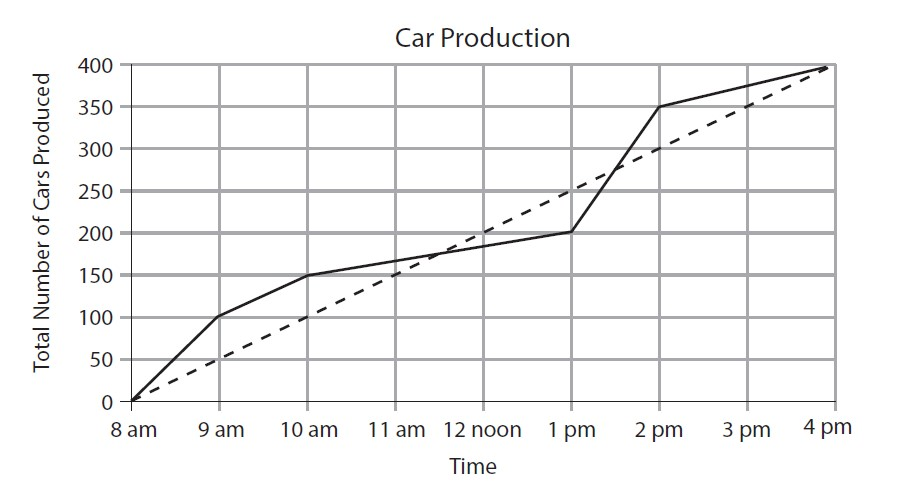
\includegraphics[max width=\textwidth]{2024_02_20_828ebc9d68bcc1fbb223g-73}

The solid line (-----------) on the graph shows car production by the NU Car Motor Company during a particular day.

The dotted line (- - - - -) shows what the total number of cars produced would be if the rate of production were constant.

By what time had a total of 150 cars been produced?

\newpage
\section*{M032681B}

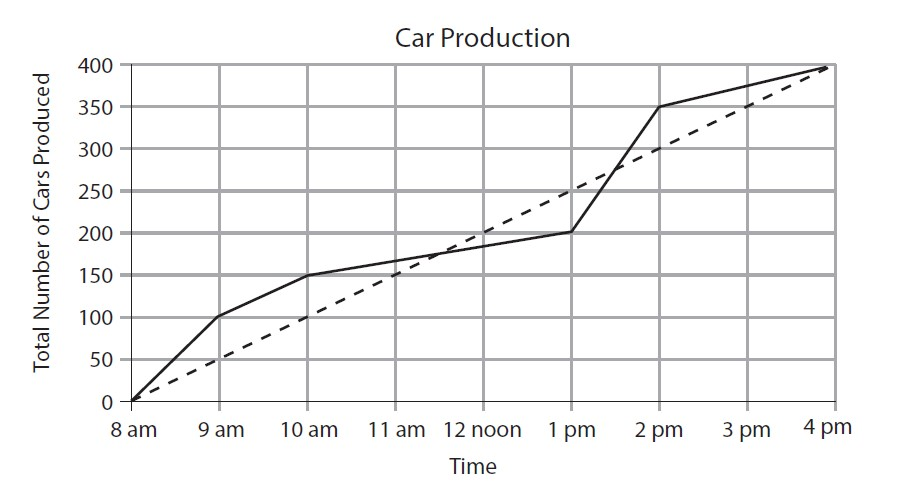
\includegraphics[max width=\textwidth]{2024_02_20_828ebc9d68bcc1fbb223g-73}

The solid line (-----------) on the graph shows car production by the NU Car Motor Company during a particular day.

The dotted line (- - - - -) shows what the total number of cars produced would be if the rate of production were constant.

What was the average number of cars produced per hour on this day?

\newpage
\section*{M032681C}

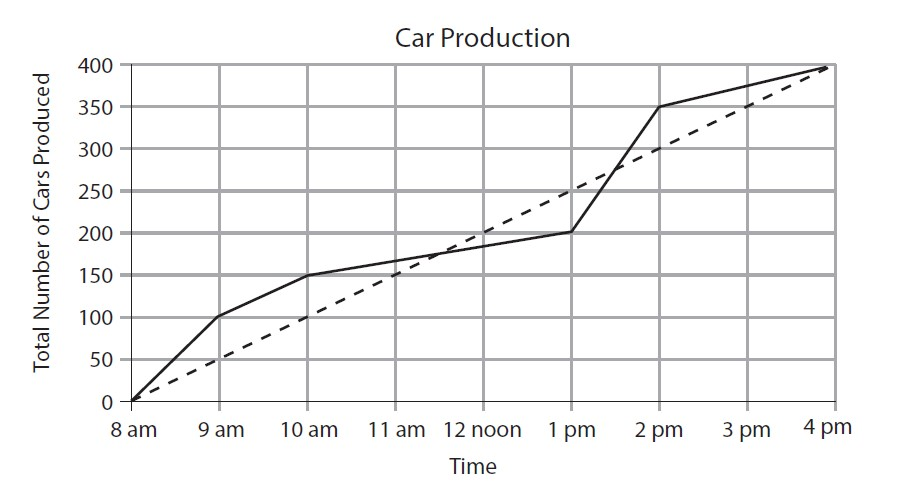
\includegraphics[max width=\textwidth]{2024_02_20_828ebc9d68bcc1fbb223g-73}

The solid line (-----------) on the graph shows car production by the NU Car Motor Company during a particular day.

The dotted line (- - - - -) shows what the total number of cars produced would be if the rate of production were constant.

During which hour were the most cars produced?


\newpage
\section*{M032695}

Of the 400 students in a school, 50 plan to go to university, 100 to a polytechnic school, 150 to a business college, and the remainder plan to enter workforce.

Use the circle below to make a pie chart showing the proportions of students planning to do each of these. Put labels on your chart.

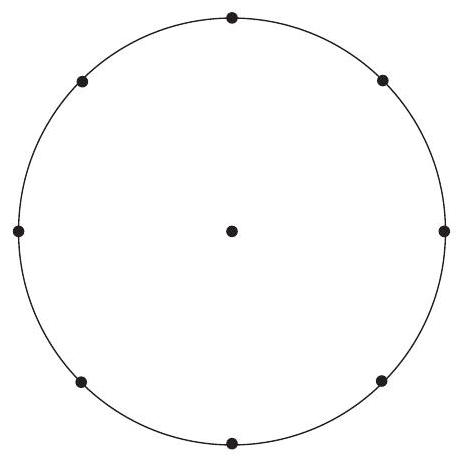
\includegraphics[max width=0.5\textwidth]{2024_02_20_828ebc9d68bcc1fbb223g-76}

\newpage
\section*{M032721}

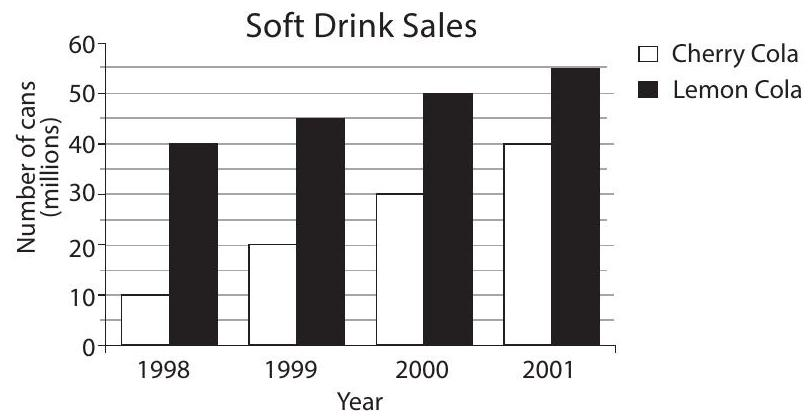
\includegraphics[max width=0.7\textwidth]{2024_02_20_828ebc9d68bcc1fbb223g-77}

The graph shows the sales of two types of soft drink over 4 years. If the sales trends continue for the next 10 years, determine the year in which the sales of Cherry Cola will be the same as the sales of Lemon Cola.

[A] 2003

[B] 2004

[C] 2005

[D] 2006

\newpage
\section*{M042169A}

The Real Burger Company owns 5 restaurants. The numbers of staff members employed in its 5 restaurants are: $12,18,19,21$, and 30 people.

What is the mean number of staff members in the 5 restaurants?

\newpage
\section*{M042169B}

The Real Burger Company owns 5 restaurants. The numbers of staff members employed in its 5 restaurants are: $12,18,19,21$, and 30 people.

What is the median number of staff members in the 5 restaurants?

\newpage
\section*{M042169C}

The Real Burger Company owns 5 restaurants. The numbers of staff members employed in its 5 restaurants are: 12, 18, 19, 21, and 30 people.

If the restaurant with 30 staff members increased its number of staff members to 50 , how would this affect the median and the mean?

\newpage
\section*{M042177}

Over recent weeks, a shop's average sales of bottles of soda have been $50 \%$ in the regular size, $40 \%$ in the small size, and $10 \%$ in the large size. Next week, the shopkeeper will order 1,200 bottles of soda. How many of these bottles should he order in the regular size?

[A] 120

[B] 480

[C] 600

[D] 720

\newpage
\section*{M042179}

There are 10 red, 8 blue, and 4 white buttons in a bag. What is the chance of taking out either a blue button or a white button?


[A] $\frac{4}{22}$ 

[B] $\frac{8}{22}$ 

[C] $\frac{10}{22}$ 

[D] $\frac{12}{22}$


\newpage
\section*{M042207}

480 students were asked to name their favorite sport. The results are shown in this table.


\begin{tabular}{|l|r|}
\hline
\multicolumn{1}{|c|}{Sport} & Number of Students \\
\hline
Hockey & 60 \\
\hline
Football & 180 \\
\hline
Tennis & 120 \\
\hline
Basketball & 120 \\
\hline
\end{tabular}


Use the information in the table to complete and label this pie chart.

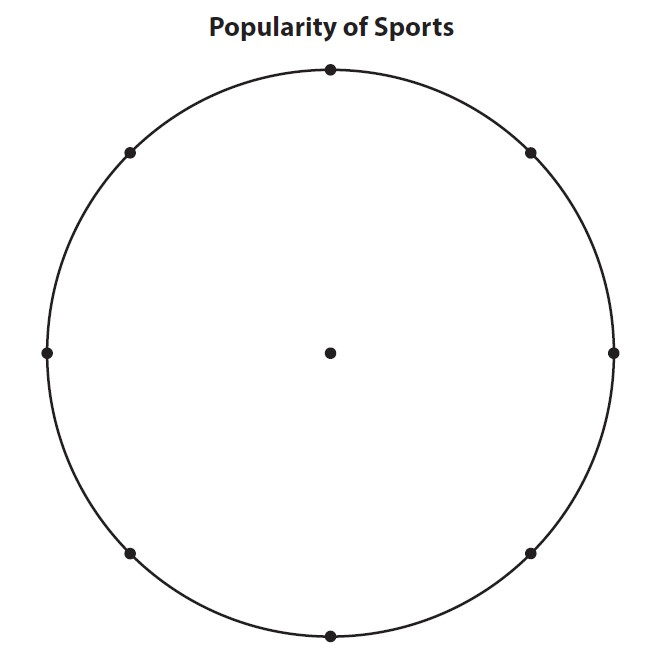
\includegraphics[max width=0.6\textwidth]{2024_02_20_828ebc9d68bcc1fbb223g-83}

\newpage
\section*{M042260}

Pat and Chris were candidates for school president.

Here are the election results:

$$
\begin{array}{ll}
\text { Pat } & 80 \% \\
\text { Chris } & 20 \%
\end{array}
$$

How likely would it be for a student asked at random to have voted for Pat?

[A] It is certain that the student voted for Pat.

[B] It is likely that the student voted for Pat.

[C] It is unlikely that the student voted for Pat.

[D] It is certain that the student did not vote for Pat.

\newpage
\section*{M042269}

The results of a long jump competition were reported as follows:

Average Length

Team A $\quad 3.6 \mathrm{~m}$

Team B $\quad 4.8 \mathrm{~m}$

There were the same number of students in each team.

Which statement about the competition MUST be true?

[A] Each student in team B jumped farther than any student in team A.

[B] After every student in team A jumped, there was a student in team B who jumped farther.

[C] As a group, team B jumped farther than team A.

[D] Some students in team A jumped farther than some students in team B.

\newpage
\section*{M052429}

There are 10 marbles in a bag: 5 red, and 5 blue.

Sue draws a marble from the bag at random. The marble is red.

She puts the marble back into the bag.

What is the probability that the next marble she draws at random is red?

[A] $\frac{1}{2}$

[B] $\frac{4}{10}$

[C] $\frac{1}{5}$

[D] $\frac{1}{10}$

\newpage
\section*{M052503A}

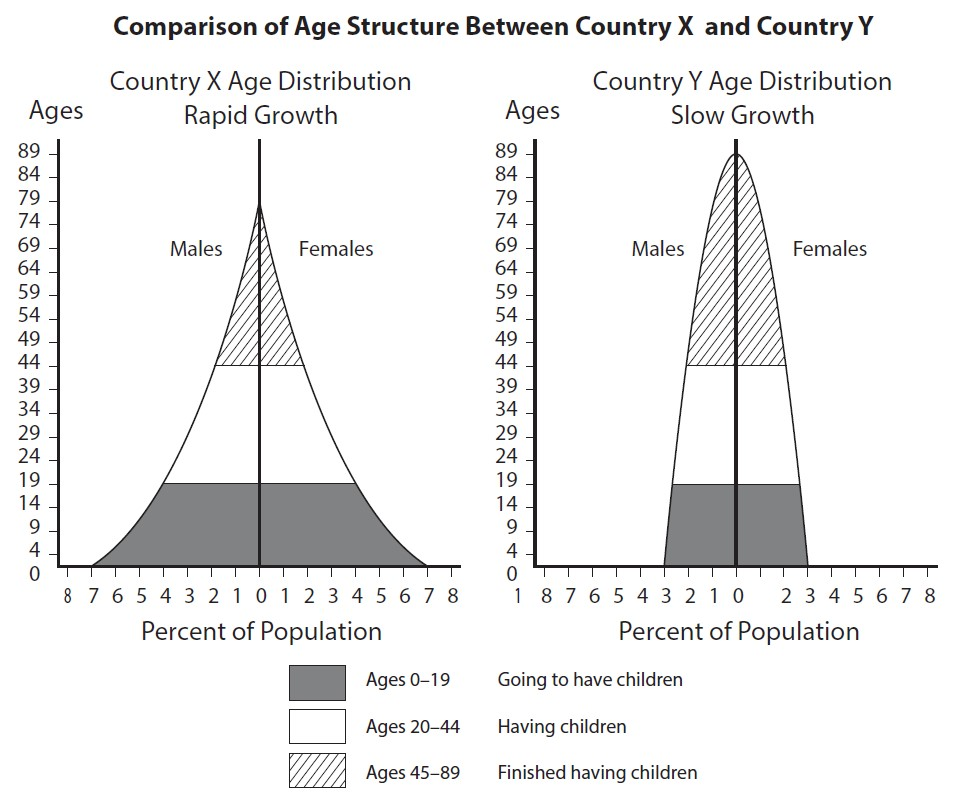
\includegraphics[max width=\textwidth]{2024_02_20_828ebc9d68bcc1fbb223g-87}

The graphs for Country $\mathrm{X}$ and Country $\mathrm{Y}$ show the age structure of each country's population. The population is divided into three age groups from youngest to oldest. The graphs enable predictions about population growth.

Why could the age structure of Country $\mathrm{X}$ lead to more rapid population growth than the age structure of Country Y?

\newpage
\section*{M052503B}

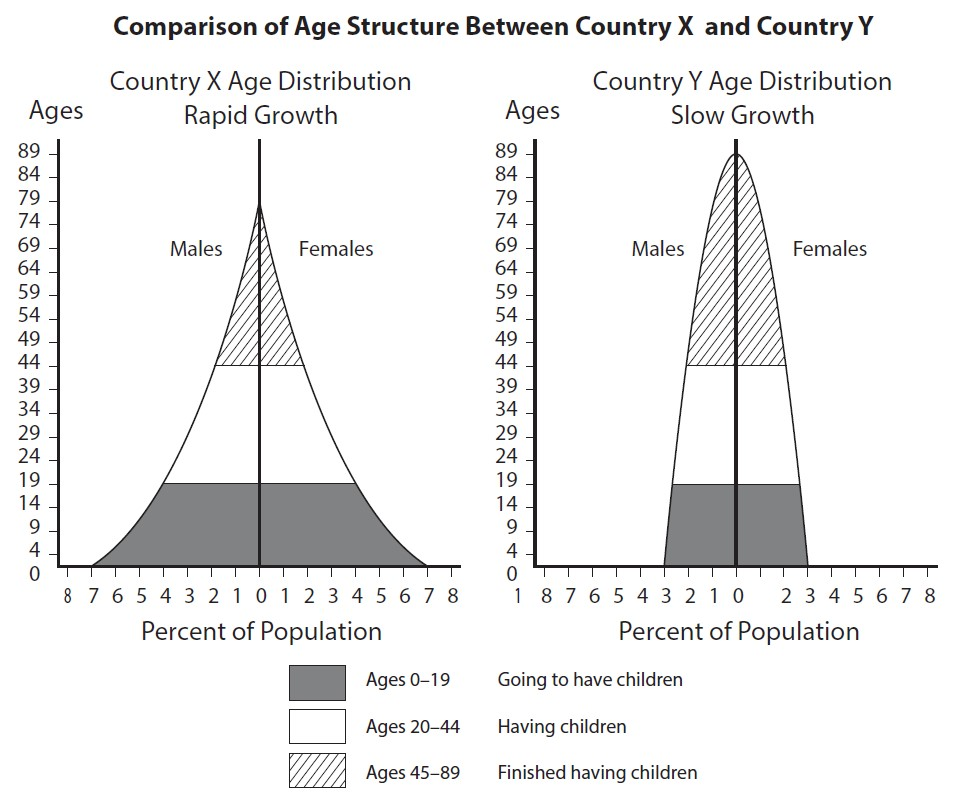
\includegraphics[max width=\textwidth]{2024_02_20_828ebc9d68bcc1fbb223g-87}

The graphs for Country $\mathrm{X}$ and Country $\mathrm{Y}$ show the age structure of each country's population. The population is divided into three age groups from youngest to oldest. The graphs enable predictions about population growth.

Why could Country Y expect to have a bigger problem taking care of its elderly population than Country X?


\end{document}